\begin{figure*}[t]
\centering
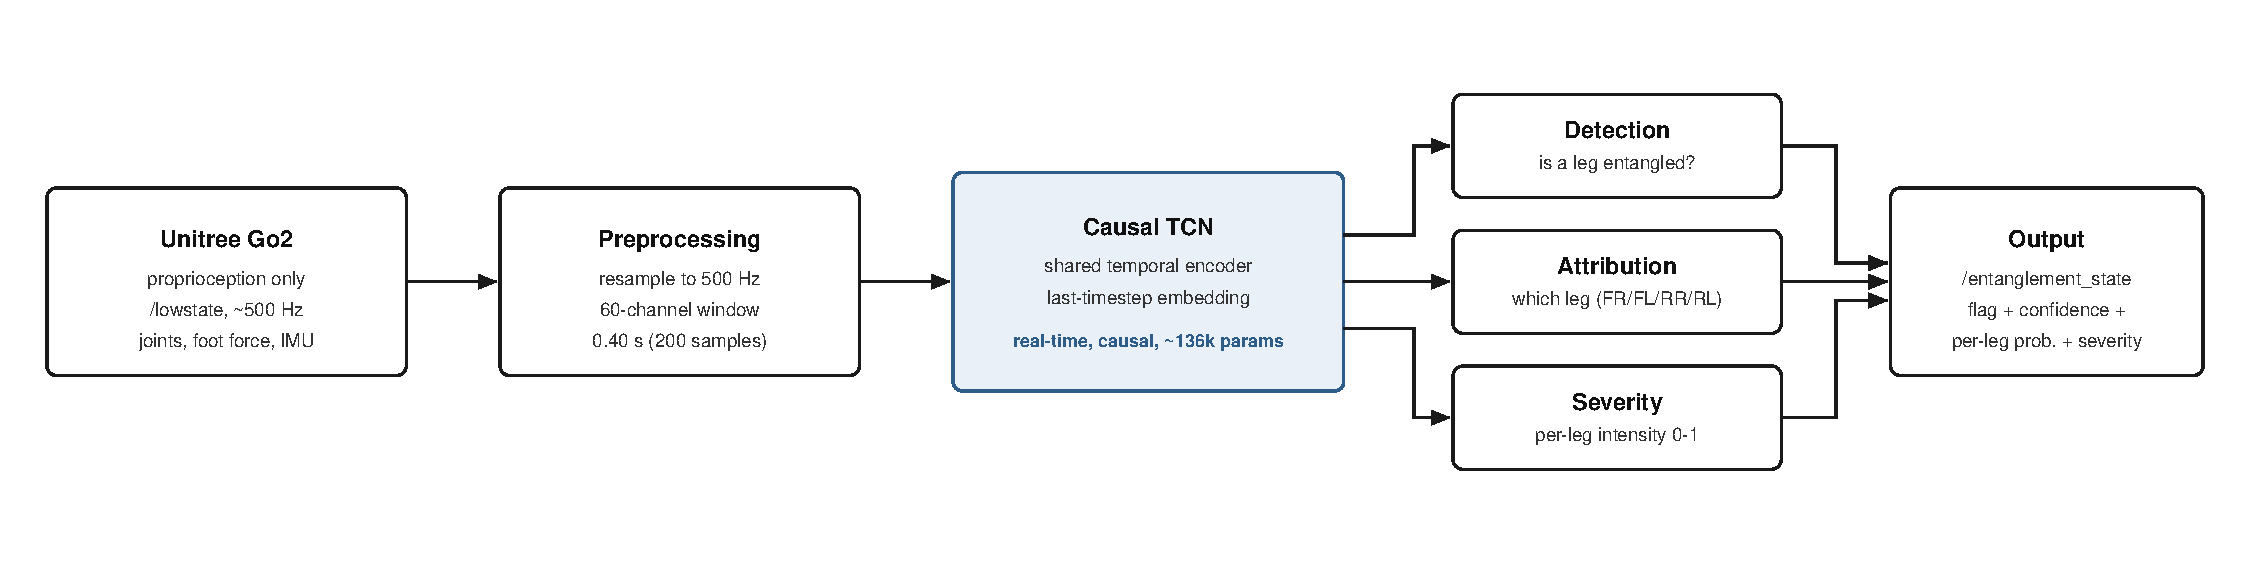
\includegraphics[width=\textwidth]{figures/fig1_system.pdf}
\caption{Overall system architecture. Proprioception from the Go2 is windowed and passed through a
shared causal TCN encoder whose three heads answer whether a leg is entangled, which leg, and how
severely; the result is published as a single state estimate.}
\label{fig:system}
\end{figure*}

\begin{figure*}[t]
\centering
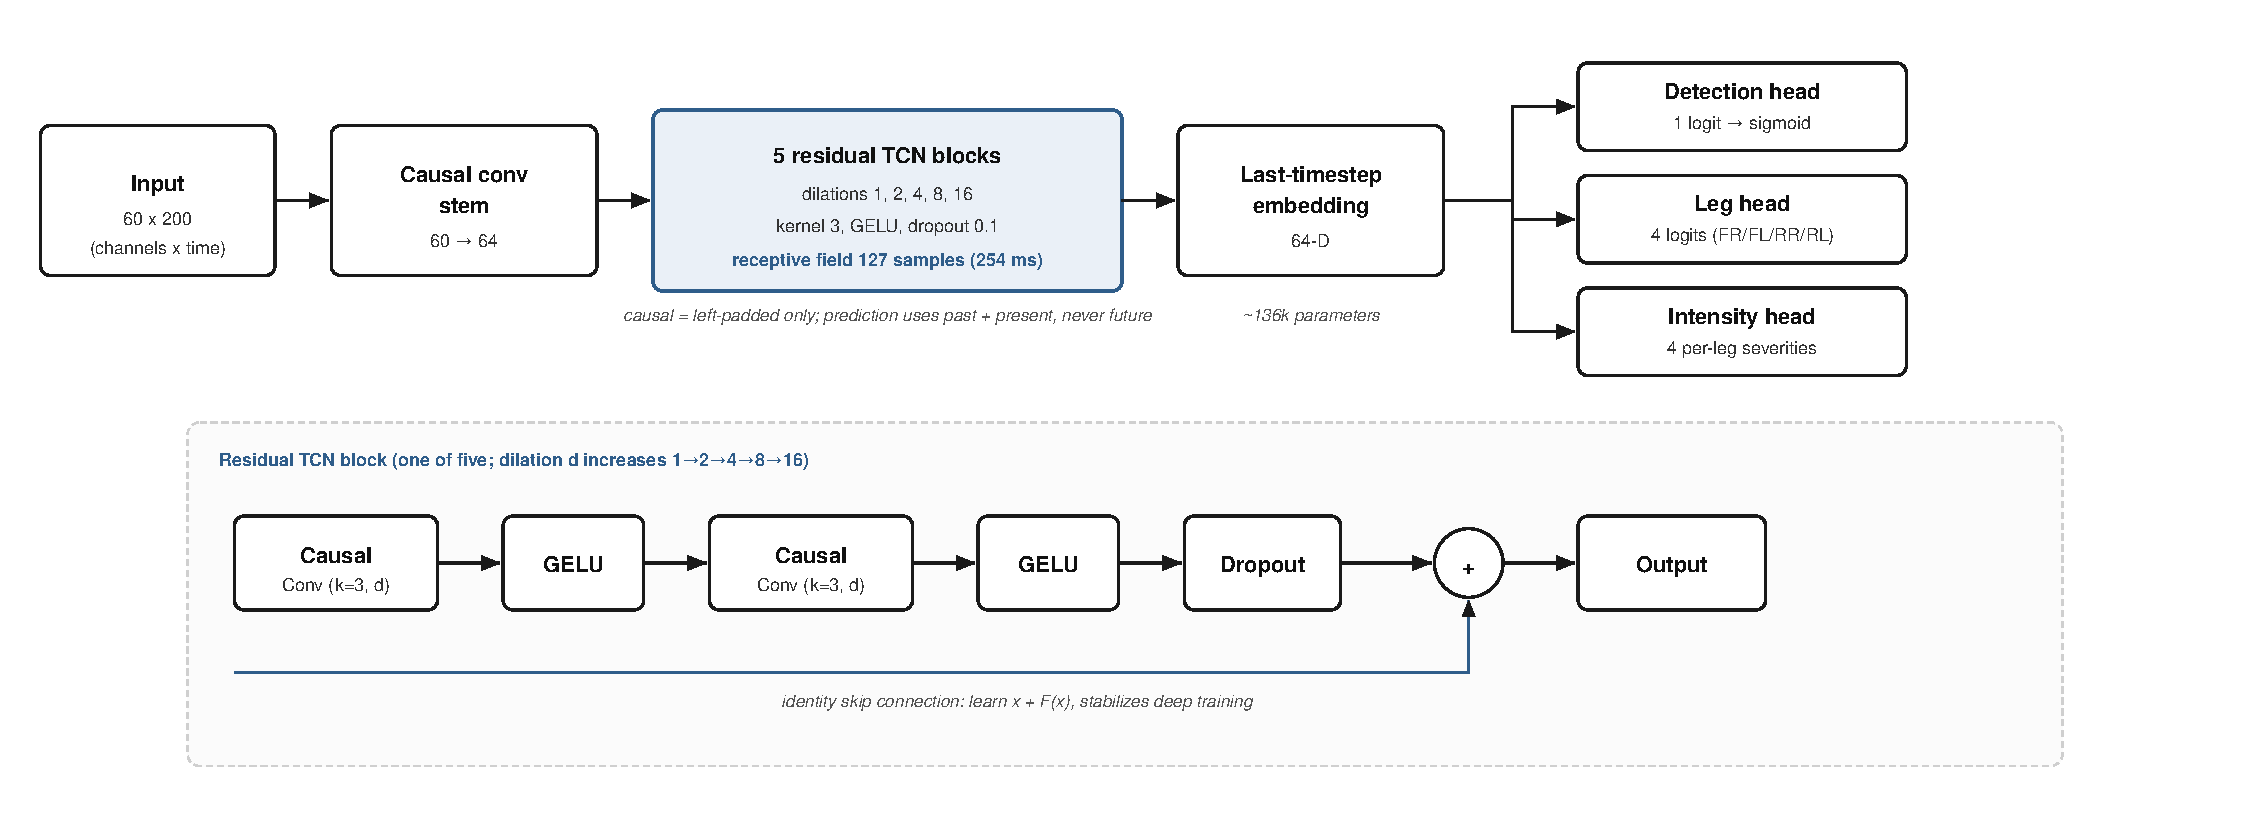
\includegraphics[width=\textwidth]{figures/fig4_tcn.pdf}
\caption{Multi-task causal TCN. A causal convolutional stem feeds five dilated residual blocks; the
last-timestep 64-D embedding drives the detection, leg-attribution, and intensity heads. The inset
shows one residual block.}
\label{fig:tcn}
\end{figure*}

\begin{figure*}[t]
\centering

\includegraphics[width=\textwidth]{figures/loro_folds.pdf}
\caption{Leave-one-recording-out cross-validation (15 folds). Bars are per-fold detection F1; the
line and band are the mean and $\pm$one standard deviation. The weakest folds are the
under-represented front-right and rear-right stop/intensity recordings.}
\label{fig:loro}
\end{figure*}

\begin{figure*}[t]
\centering

\includegraphics[width=\textwidth]{figures/field_issues.pdf}
\caption{Deployment robustness from targeted data augmentation. (a) Three false-firing modes fall to
zero. (b) Front-right detection rises from near zero to full. Values are per-phase firing percentages
on the named recordings.}
\label{fig:field}
\end{figure*}

\begin{table}[t]
\centering
\caption{Dataset composition. 25 recordings, 159{,}001 labeled rows, logged non-uniformly
($\approx$410--500\,Hz, median $\approx$483\,Hz) and resampled to 500\,Hz at the feature stage. The
affected leg is encoded in the file name.}
\label{tab:dataset}
\footnotesize
\begin{tabular}{@{}lccl@{}}
\toprule
Scenario & \#Rec. & Affected & Interaction \\
\midrule
\texttt{back\_both}  & 2 & RR, RL & wire \\
\texttt{back\_left}  & 3 & RL     & hand / wire \\
\texttt{back\_right} & 3 & RR     & hand / wire \\
\texttt{front\_both} & 2 & FR, FL & wire \\
\texttt{front\_left} & 2 & FL     & hand \\
\texttt{front\_right}& 1 & FR     & wire \\
\texttt{back\_right} (at rest) & 2 & RR & wire \\
\midrule
\texttt{walking} & 5 & --- & normal gait \\
\texttt{stop}    & 3 & --- & standing \\
\texttt{lock\_stop}, \texttt{walk\_stop\_back} & 2 & --- & Lock / backward \\
\midrule
\textbf{Total} & \textbf{25} & \multicolumn{2}{l}{\textbf{15 positive / 10 negative}} \\
\bottomrule
\end{tabular}
\end{table}

\begin{table}[t]
\centering
\caption{The 60-channel input representation. Motor torque is the estimated joint torque $\tau$.}
\label{tab:features}
\footnotesize
\begin{tabular}{@{}llc@{}}
\toprule
Group & Channels & Count \\
\midrule
Motor & 4 legs $\times$ \{hip, thigh, calf\} $\times$ \{$q,\dot q,\tau$\} & 36 \\
Foot force & one per leg & 4 \\
IMU & roll, pitch, gyro$_{xyz}$, acc$_{xyz}$ (yaw dropped) & 8 \\
Engineered & per leg: 3 physics features (Sec.~\ref{sec:feat}) & 12 \\
\midrule
\textbf{Total} & & \textbf{60} \\
\bottomrule
\end{tabular}
\end{table}

\begin{table}[t]
\centering
\caption{Model and training configuration.}
\label{tab:hparams}
\footnotesize
\begin{tabular}{@{}ll@{}}
\toprule
Item & Value \\
\midrule
Window / hop (train, eval) & 200 (0.40\,s) / 25, 1 \\
Resample rate & 500\,Hz \\
Encoder width / blocks & 64 / 5 \\
Dilations; kernel; dropout & 1,2,4,8,16; 3; 0.1 \\
Receptive field & 127 samples (254\,ms) \\
Parameters & 136{,}393 \\
Loss weights (det / leg / int.) & 1.0 / 1.0 / 0.3 \\
Intensity Huber & $\delta{=}0.1$, affected-leg $3{:}1$ up-weight \\
Optimizer & AdamW, lr $10^{-3}$, wd $10^{-4}$ \\
Schedule; batch; epochs; seed & cosine; 256; 30; 1234 \\
Sampler & class-balanced, rare-leg up-weighted \\
\bottomrule
\end{tabular}
\end{table}

\begin{table}[t]
\centering
\caption{Detection on the held-out test split (raw threshold 0.9999). Both detectors are scored
under the identical protocol.}
\label{tab:detection}
\footnotesize
\begin{tabular}{@{}lcc@{}}
\toprule
Metric & Causal TCN & Rule-based (thigh torque) \\
\midrule
Precision       & \textbf{0.799} & 0.735 \\
Recall          & \textbf{0.818} & 0.131 \\
F1              & \textbf{0.809} & 0.222 \\
PR-AUC          & \textbf{0.808} & 0.639 \\
ROC-AUC         & \textbf{0.956} & 0.830 \\
Leg exact-match & \textbf{0.908} & 0.106 \\
\bottomrule
\end{tabular}
\end{table}

\begin{table}[t]
\centering
\caption{Per-leg attribution on the test split.}
\label{tab:perleg}
\footnotesize
\begin{tabular}{@{}lccc@{}}
\toprule
Leg & Precision & Recall & F1 \\
\midrule
FR & 0.467 & 1.000 & 0.636 \\
FL & 0.731 & 1.000 & 0.845 \\
RR & 0.551 & 0.959 & 0.700 \\
RL & 0.748 & 0.916 & 0.823 \\
\bottomrule
\end{tabular}
\end{table}
